\section{VideoGPT}
\label{sec:videogpt}

\begin{figure}
    \centering
    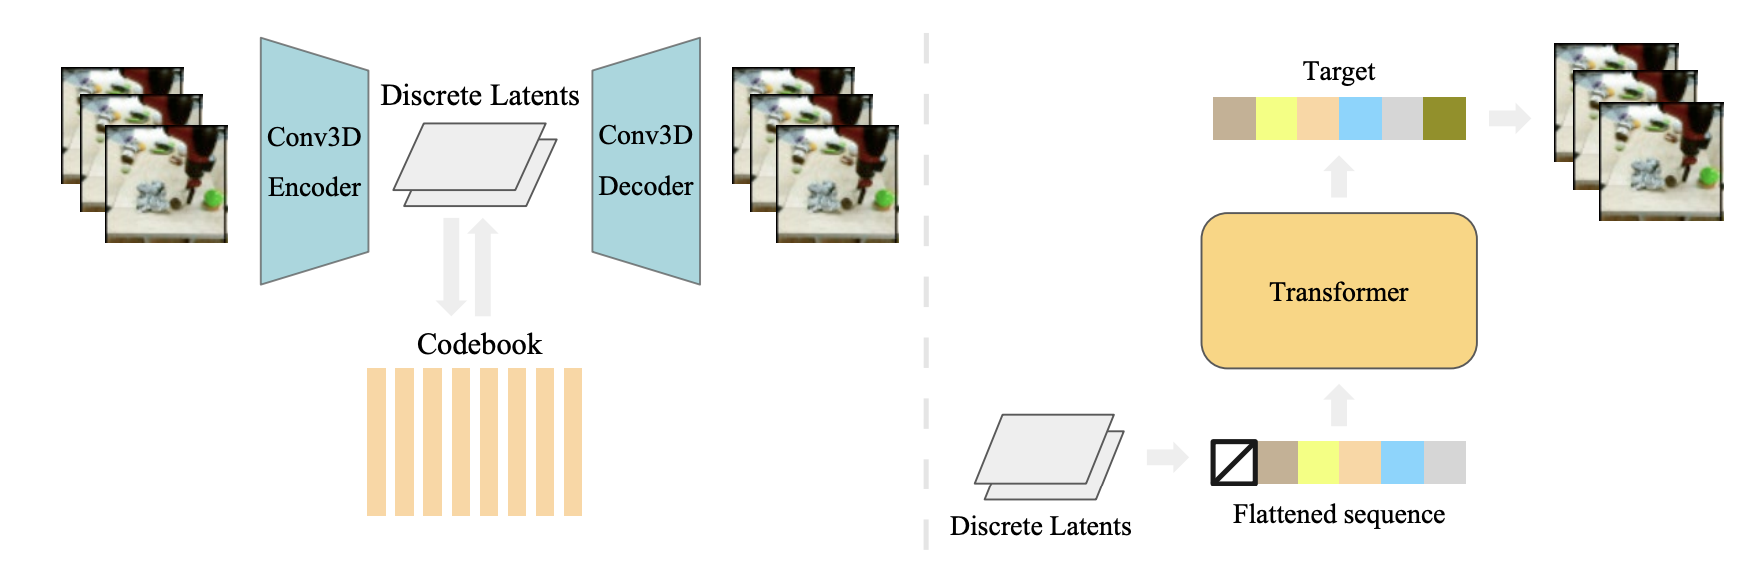
\includegraphics[width=0.7\textwidth]{images/video_synthesis/videogpt_architecture.png}
    \caption{VideoGPT architecture. Left: training the VQ-VAE; Right: training the autoregressive transformer model on the latent vectors.}
\end{figure}

VideoGPT \cite{videogpt} uses likelihood based model VQ-VAE and GPT-like transformer model. The encoder of VQ-VAE first downsamples video into discrete latent space using 3D convolutions, and the decoder then reconstructs the video from these latent codes (by using a codebook - see VQ-VAE section \ref{sec:vqvae}). The generated latents are decoded to the original video resolution as the training dataset.

The researchers take inspiration from image and video codecs: JPEG and MPEG for image and video compression. They contain the same spatio-temporal data as the uncompressed video, yet take less resources (by not working in the pixel space).

\subsection*{The VQ-VAE}

Reminder that the loss function of VQ-VAE is defined:

\begin{equation*}
    \mathcal{L} = \underbrace{\left| \left| x - D(e) \right| \right|^2_2}_{\mathcal{L}_\text{recon}} + \underbrace{\left| \left| \text{sg}\left[ E(x) \right] - e \right| \right|^2_2}_{\mathcal{L}_\text{codebook}} + \underbrace{\beta \left| \left| \text{sg}[e] - E(x) \right| \right|^2_2}_{\mathcal{L}_\text{commit}}
\end{equation*}

where $\text{sg}$ refers to stop-gradient, $\mathcal{L}_\text{recon}$ is the \textbf{reconstruction loss} (encourages the VQ-VAE to learn good representations to accurately reconstruct the data), $\mathcal{L}_\text{codebook}$ is the \textbf{codebook loss} (quantization loss, it brings codebook vectors closer to the encoder outputs), and $\mathcal{L}_\text{commit}$ is the \textbf{commitment loss} (which prevents the encoder outputs from fluctuating between different code vectors). 

The reconstruction loss optimizes only the decoder, the commitment loss optimizes only the encoder, and the codebook loss optimizes the codebook embeddings only. See section \ref{sec:vqvae} for more details.

The researchers used EMA (exponential moving average which is described in the VQ-VAE paper \cite{vqvae}) update for the codebook loss. In short, it makes the VQ-VAE faster to train and converge.

\begin{figure}
    \centering
    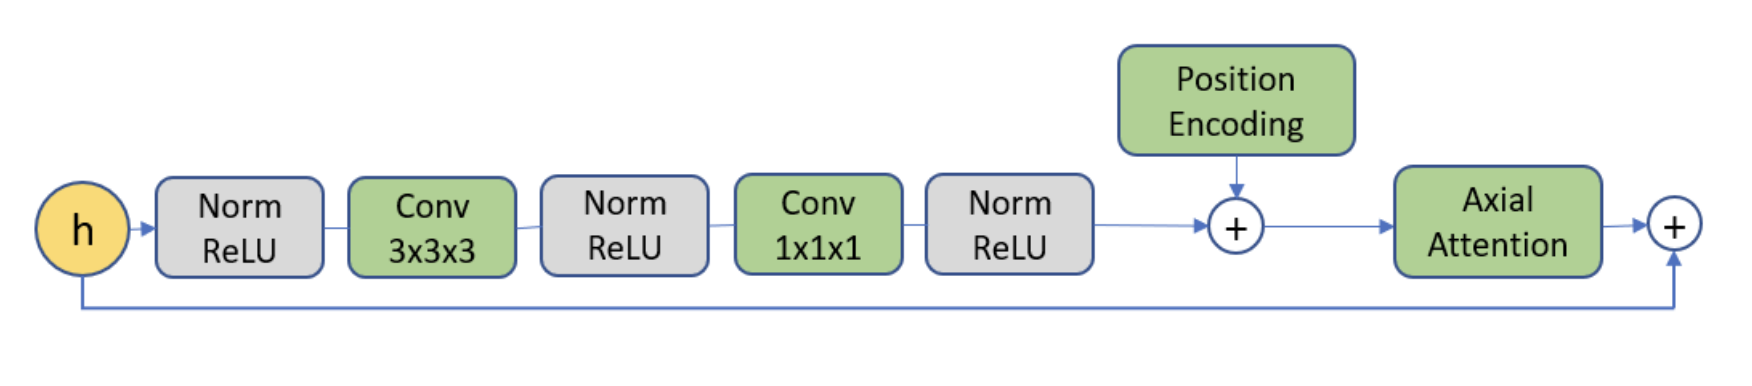
\includegraphics[width=0.6\textwidth]{images/video_synthesis/videogpt_res_atten_block.png}
    \caption{Residual attention block as described in VideoGPT. The "Norm" layers are \texttt{LayerNorm} blocks (described in appendix \ref{appendix:blocks_norm}).}
    \label{fig:videogpt_res_atten_block}
\end{figure}

To train the VQ-VAE model (to learn the latent codes), the authors trained the VQ-VAE on video data. The encoder consists of downsample 3D convolutions (appendix \ref{appendix:blocks_3dconv}) followed by attention residual blocks (figure \ref{fig:videogpt_res_atten_block}), and they used \texttt{LayerNorm}.

The architecture of the \textbf{decoder} is the reverse of the encoder (residual attention blocks followed by upscale 3D convolutions).

\subsection*{The transformer (GPT)}

As described in section \ref{sec:vqgan}, GPT is autoregressive transformer model. The autoregressive nature can be described as $p(x) = \prod_{i=1}^{d} p(x_i | x_{\leq i})$ through masked self-attention. The GPT transformer is optimized through maximum likelihood (appendix \ref{appendix:likelihood_function}). 






\subsection{Architecture}

They train the VQ-VAE on video data to learn the codebook. The encoder and decoder consists of 3D convolutions (appendix \ref{appendix:blocks_3dconv}) followed by attention residual blocks (figure \ref{fig:videogpt_res_atten_block}). Axial attention block is described in appendix \ref{appendix:attention}.